\documentclass[11pt]{article}
\usepackage[utf8]{inputenc}
\usepackage{setspace}
\usepackage[colorlinks]{hyperref}
\usepackage{lineno}
\usepackage{natbib}
\usepackage{booktabs}
\usepackage{graphicx}
\usepackage{float}
\usepackage{subfigure}
\usepackage[justification=centering]{caption}
\usepackage{amsmath}

\title{NLLS Models Generally Outperform OLS Models for Quantifying Microbial Population Growth Data}

\author{Shengge Tong (shengge.tong22@imperial.ac.uk)}

\date{Dec,2022}


\linespread{1.5}
\begin{document}
\begin{titlepage}

  \centering

    \vspace*{3cm}
    \Huge
    \textbf{NLLS Models Generally Outperform OLS Models for Quantifying Microbial Population Growth Data}\\
    
    \vspace*{2cm}
    \Large
    \textbf{Author:} Shengge Tong (shengge.tong22@imperial.ac.uk)\\
    \vspace*{1cm}
    \textbf{Word Count:1323} 

  \end{titlepage}
\newpage
\tableofcontents
\newpage
\addcontentsline{toc}{section}{Abstract}
 
  \begin{abstract}
    The abundance (density) of a single population may be critical to determining ecosystem dynamics and functional characteristics. And microbial (specifically, bacterial) growth rates is a hot research topic.
    This report focus on the model fitting and comparison of the population growth data. There are four models in the study, including OLS(Quadratic polynomial and Cubic polynomial) and NLLS (Logistic and Gompertz) models. The study tries to find the best model by comparing the $AIC$, $AIC_c$, $R^2$ (three measurements). 
    The results showed that Gompertz model had best performance on fitting the data. Logistic model is sufficient for the simple growth case. OLS models are suitable for simple cases.
    In conclusion, Gompertz should be preferred if extreme performance is sought, as the model has more parameters and a relatively low probability of convergence, it may require more potential labor costs to adjust the initial values.
    \newline
  \end{abstract}
\newpage

 \section{Introduction}
 Human society has a strong correlation with microbial growth. For example, Wine fermentation cannot be done without yeast, mold can make food spoiled, pneumococcus can make people sick, and some probiotics can keep people's intestinal health.
  There are four periods for bacterial growth:
  \newline
  (1) lag phase: After inoculation of the bacteria into the medium, there is a short adaptation process to the new environment (those that do not adapt can die due to the transfer). The curve is flat and stable during this period, as the bacteria multiply very little.
  \newline
  (2) logarithmic phase: The number of viable bacteria on the growth curve increases linearly during this period. The bacteria grow very rapidly in a steady geometric progression that can last from a few hours to a few days. The morphology, staining and biological activity of bacteria in this stage are typical and sensitive to the action of external environmental factors, so the study of bacterial traits is best in this stage.
  \newline
  (3) stationary phase: The total number of growing colonies in this period was in a flat phase, but the bacterial population viability was highly variable. The number of bacterial proliferations and deaths were gradually balanced in this period.
  \newline
  (4) decline phase: Bacteria multiply more and more slowly, and the number of dead bacteria increases significantly. The number of live bacteria is inversely related to the incubation time, the bacteria become long and swollen or deformed decay in this period, and the physiological metabolic activities tend to stagnate.
 
  There are many mathematical models could be used to predict the growth curve. According to the past research and study, some NLLS models such as modifed Gompertz model (\citealt{PMID:16348228}), Logistic model(\citealt{MARCHETTI19961}) are widely used in this field.
  And our goal is to compare the OLS models (Cubic, Quadratic)(\citealt{SAKANOUE2007159})(\citealt{GELADI19861}) with NLLS models by $AIC$, $AIC_c$, $R^2$ (\citealt{10.1093/biomet/78.3.499}).
  Thus, this report is mainly about which model has the best performance, and illustrate their pros and cons. Finally, a good strategy could be made for fitting the data in different cases.
 \section{Data and Methods}

  \subsection{Data Preparation}
    The raw dataset for project is LogisticGrowthData.csv. And the field names are in LogisticGrowthMetaData.csv. They are both in the data directory.
    This project mainly focus on the relation between PopBio(abundance) with Time. Firstly, I loaded the data and combined Species, Medium, Temp and Citation columns to set up the ID coulmns. Secondly, I filtered the data for Time and PopBio larger than 0, removing meaningless data. Then I seperated them into several groups to get 256 independent experiments.

  \subsection{Models} 
    
    There are 4 models to be used in the project. Polynomial models and Logistic model are fitted with non-logged data, and Gompertz model with logged data. 
    Here are the formulas of each model. $T$ is the time variable. $LogPopBio(T)$ is the $ln$(abundance) of $T$. $N_0$ is initial population size, $r_{max}$ is the maximum growth rate , and $N_{Max}$ is carrying capacity (commonly denoted by $K$ in the ecological literature).
\newline 
Quadratic polynomial model 
\begin{equation} PopBio(T) = A_0 + A_1 T + A_2 T^2 \end{equation}  \\ 
Cubic polynomial model
\begin{equation} PopBio(T) = A_0 + A_1 T + A_2 T^2 + A_3 T^3 \end{equation}  \\      
Logistic model 
\begin{equation} PopBio(T) = \frac{N_0 N_{Max} e^{r_{max} t}}{N_{Max}+N_0(e^{r_{max} t} - 1)}\end{equation} \\ 
Gompertz model
\begin{equation} LogPopBio(T) = N_O + (N_{Max} - N_0) e^{-e^{\frac{r_{max}  e^1  (t_{lag} - T)}{(N_{Max} - N_0)  log(10)} + 1 }}\end{equation} \\

\subsection{Computing Tools}   
\emph{Python 3.10.6} was used to do data preprocessing and model fitting. The packages \emph{pandas} and \emph{numpy} were used to preprocess the data. The \emph{matplotlib} and\emph{seaborn} were used to plot the data. The \emph{scipy}, \emph{sklearn} and \emph{lmfit} were used to fit models. And \emph{warnings} was used to ignore the warnings.
\emph{Bash} was used to run all the Python and LaTex scripts.

\subsection{Model Fitting} 
  For NLLS model, especially Gompertz, it is very important to determine the starting value. As the Gompertz has quite a large number of parameters: $N_0$, $N_{max}$, $r_{max}$, $t_{lag}$, the probability of model convergence is relatively low. For partial ID prediction, the initial value of the model needs to be continuously adjusted to converge. However, Linear (OLS) models do not care the starting value.
    
\subsection{Model Selection}
  Three statistical methods($AIC$, $AIC_c$, $R^2$) were used in this study to measure the performance of the models. The following show the equations of them:
  
  \begin{equation} 
  AIC = 2k - 2ln(L)
  \end{equation} 

  \begin{equation} 
  AIC_c = AIC + \frac{2k(k+1)}{n-k-1}
  \end{equation} 

  \begin{equation} 
  R^2 = 1 - \frac{SSR}{SST}
  \end{equation} 
  $k$ is the number of parameters and $L$ is the likelihood function. A small $k$ implies a concise model and a large $L$ implies an accurate model, so the model is evaluated with a balance of conciseness and accuracy.
  In the case of small samples, $AIC$ transforms to $AIC_c$. So $AIC_c$ can be applied to any sample size.
  $R^2$ is generally used in regression to assess how good or bad the model is. The closer the value is to 1, the better the model performance is, and less than 0, it usually means that the model is very poor.
  
 \newpage
 \section{Results}
After filtering the data (by $Data Preparation$), I got 256 sets in total for the model fitting. I got each models' fitting results and output the $AIC$, $AIC_c$, $R^2$ distributions in $results$ directory. Besides, I ploted each set of fitting results in the $sandbox$ directory.
  \subsection{Model Fitting Count}
    In Figure 1, it showed that the OLS models fitted most of the data, especially the Cubic Polynomial. Then the Quadratic Polynomial also fitted well. For the mechanistic models, Gompertz model fitted quite well but Logistic model only fitted half of the data successfully. 
    The mainly reason of this is that there were low count of data points in some sets, so it caused under fitting problems.

    \begin{figure}[H]
      \centering
      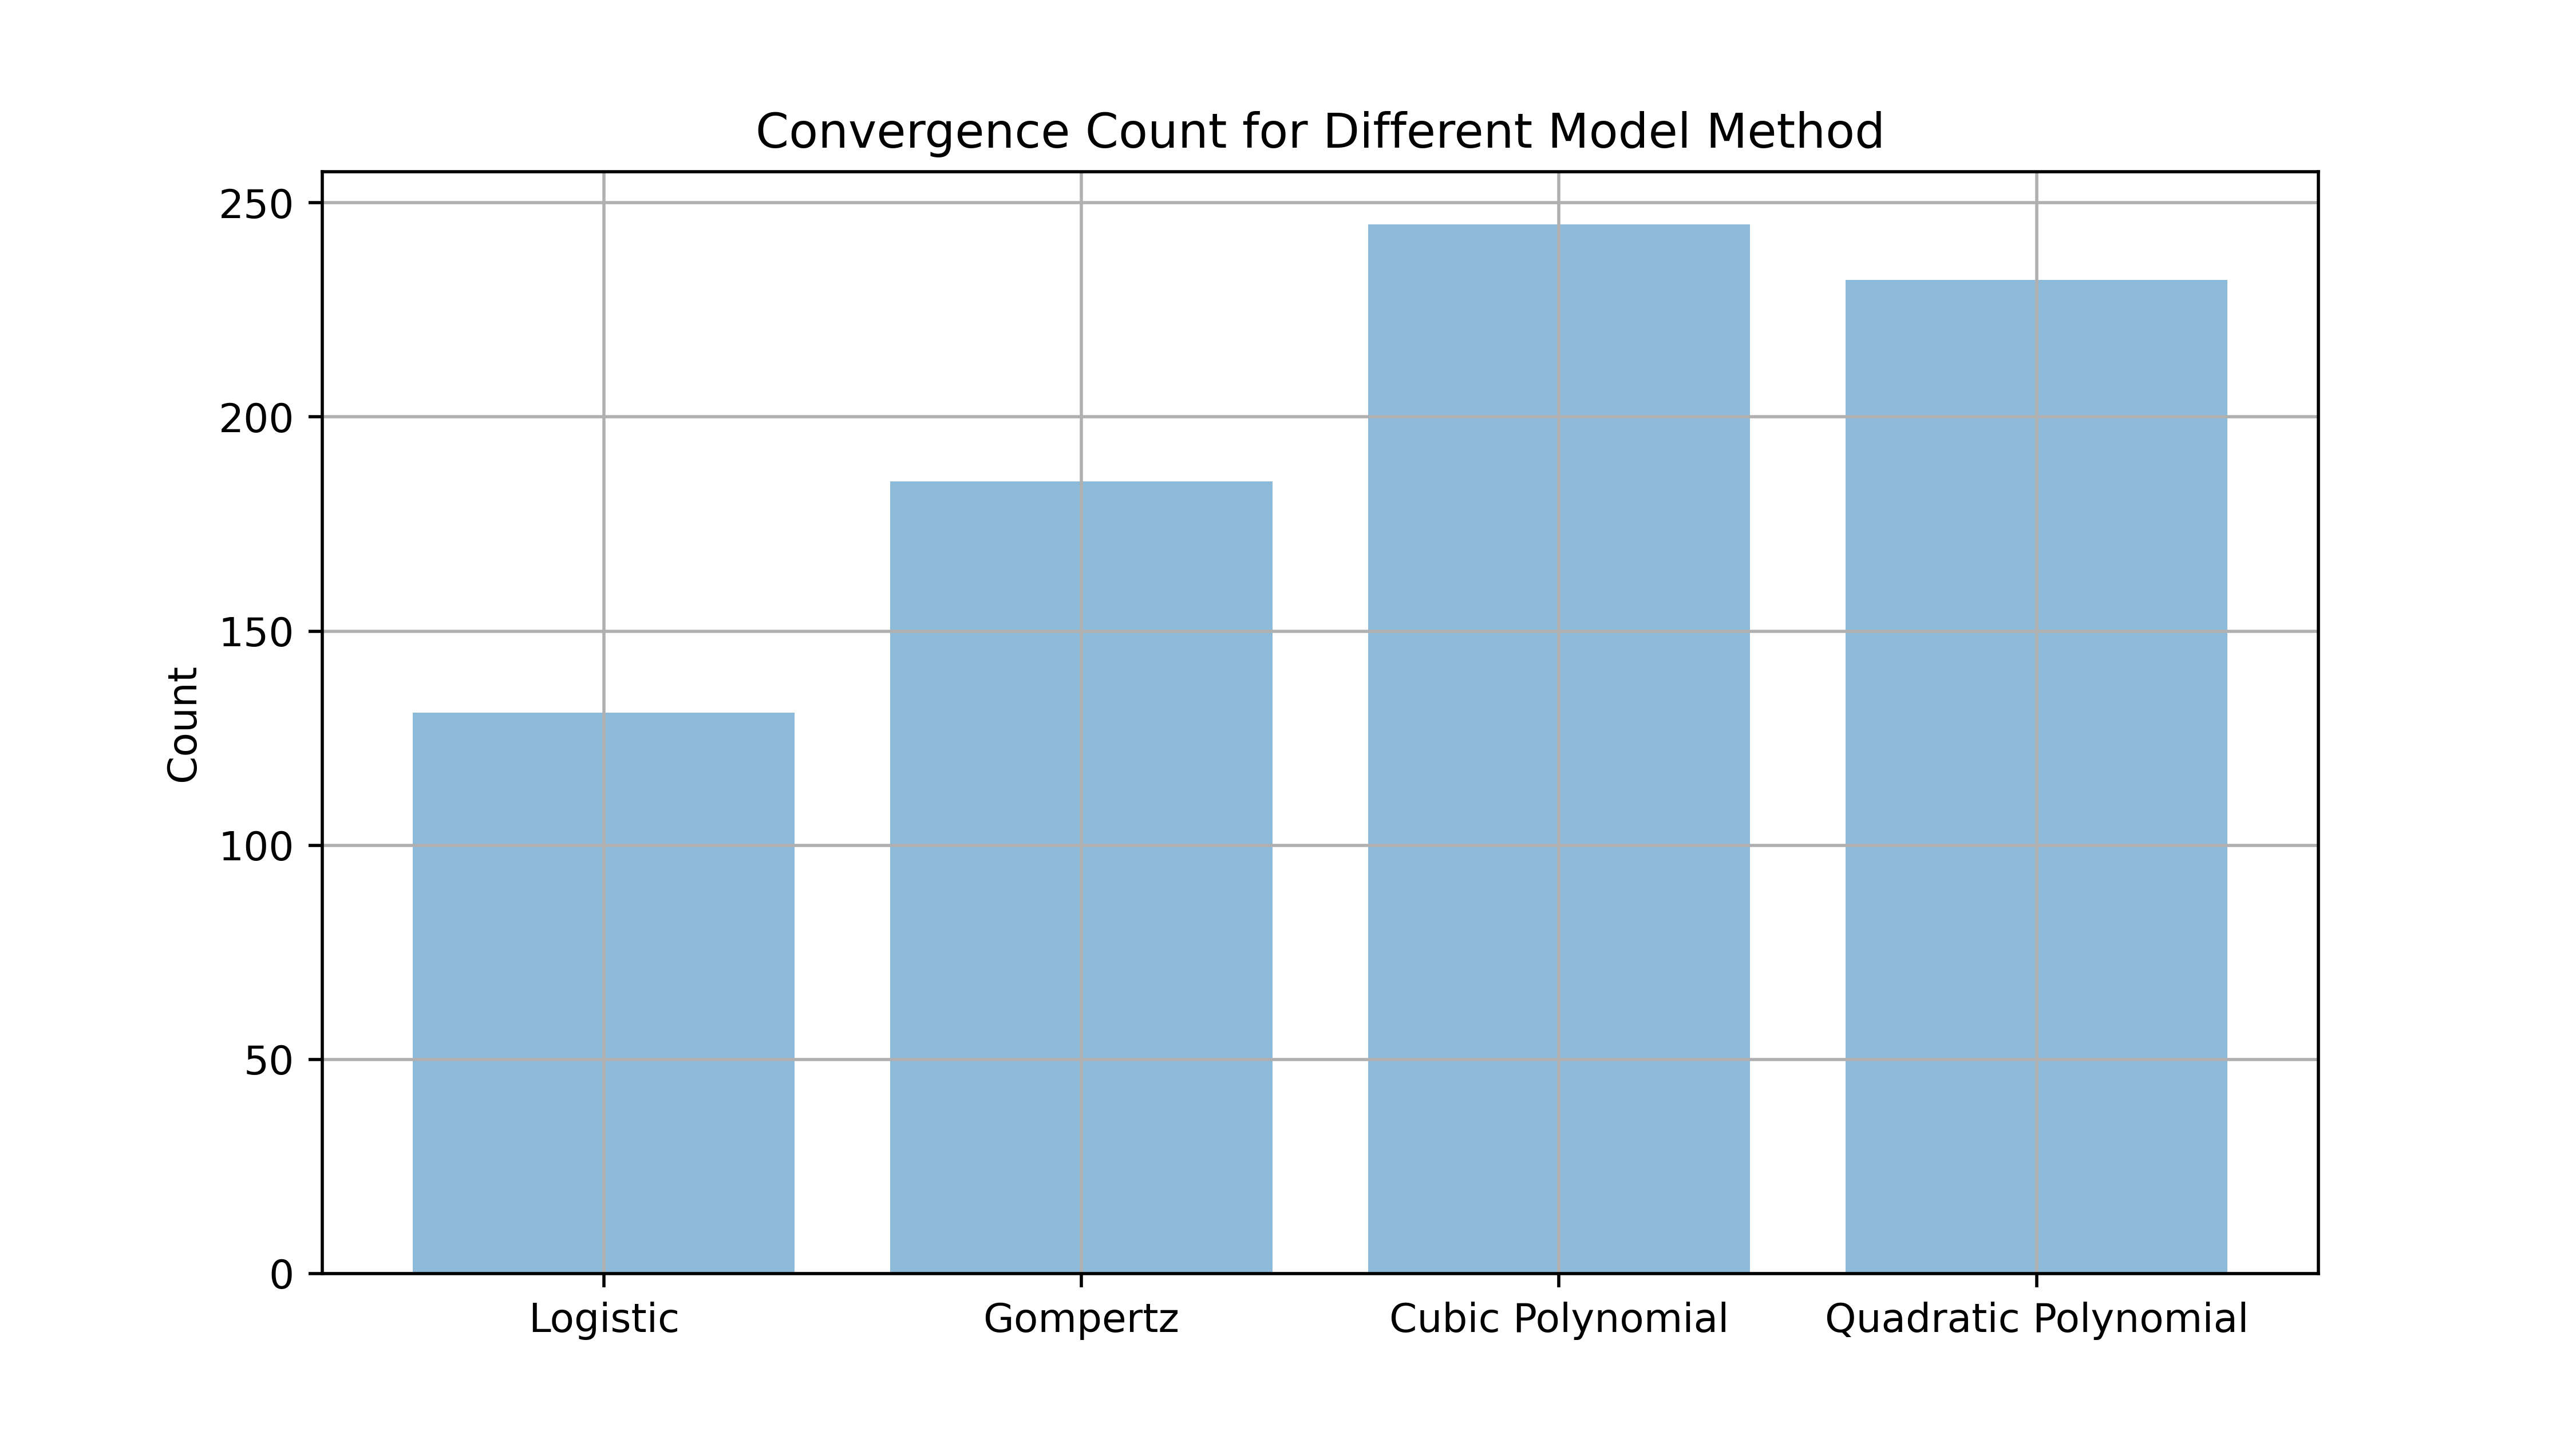
\includegraphics[width=\textwidth]{../results/Model_Convergence_Count.png}
      \caption{It showed the number of fitted models}
    \end{figure}
  
  \newpage
  \subsection{Model Comparison}
    Figure 2 showed the $R^2$ distributions of models. Figure 3 shows the descriptive statistics of $R^2$.
    By comparing the $R^2$ of the models, it illustrated that the Cubic polynomial is the best.

    \begin{figure}[H]
      \centering
      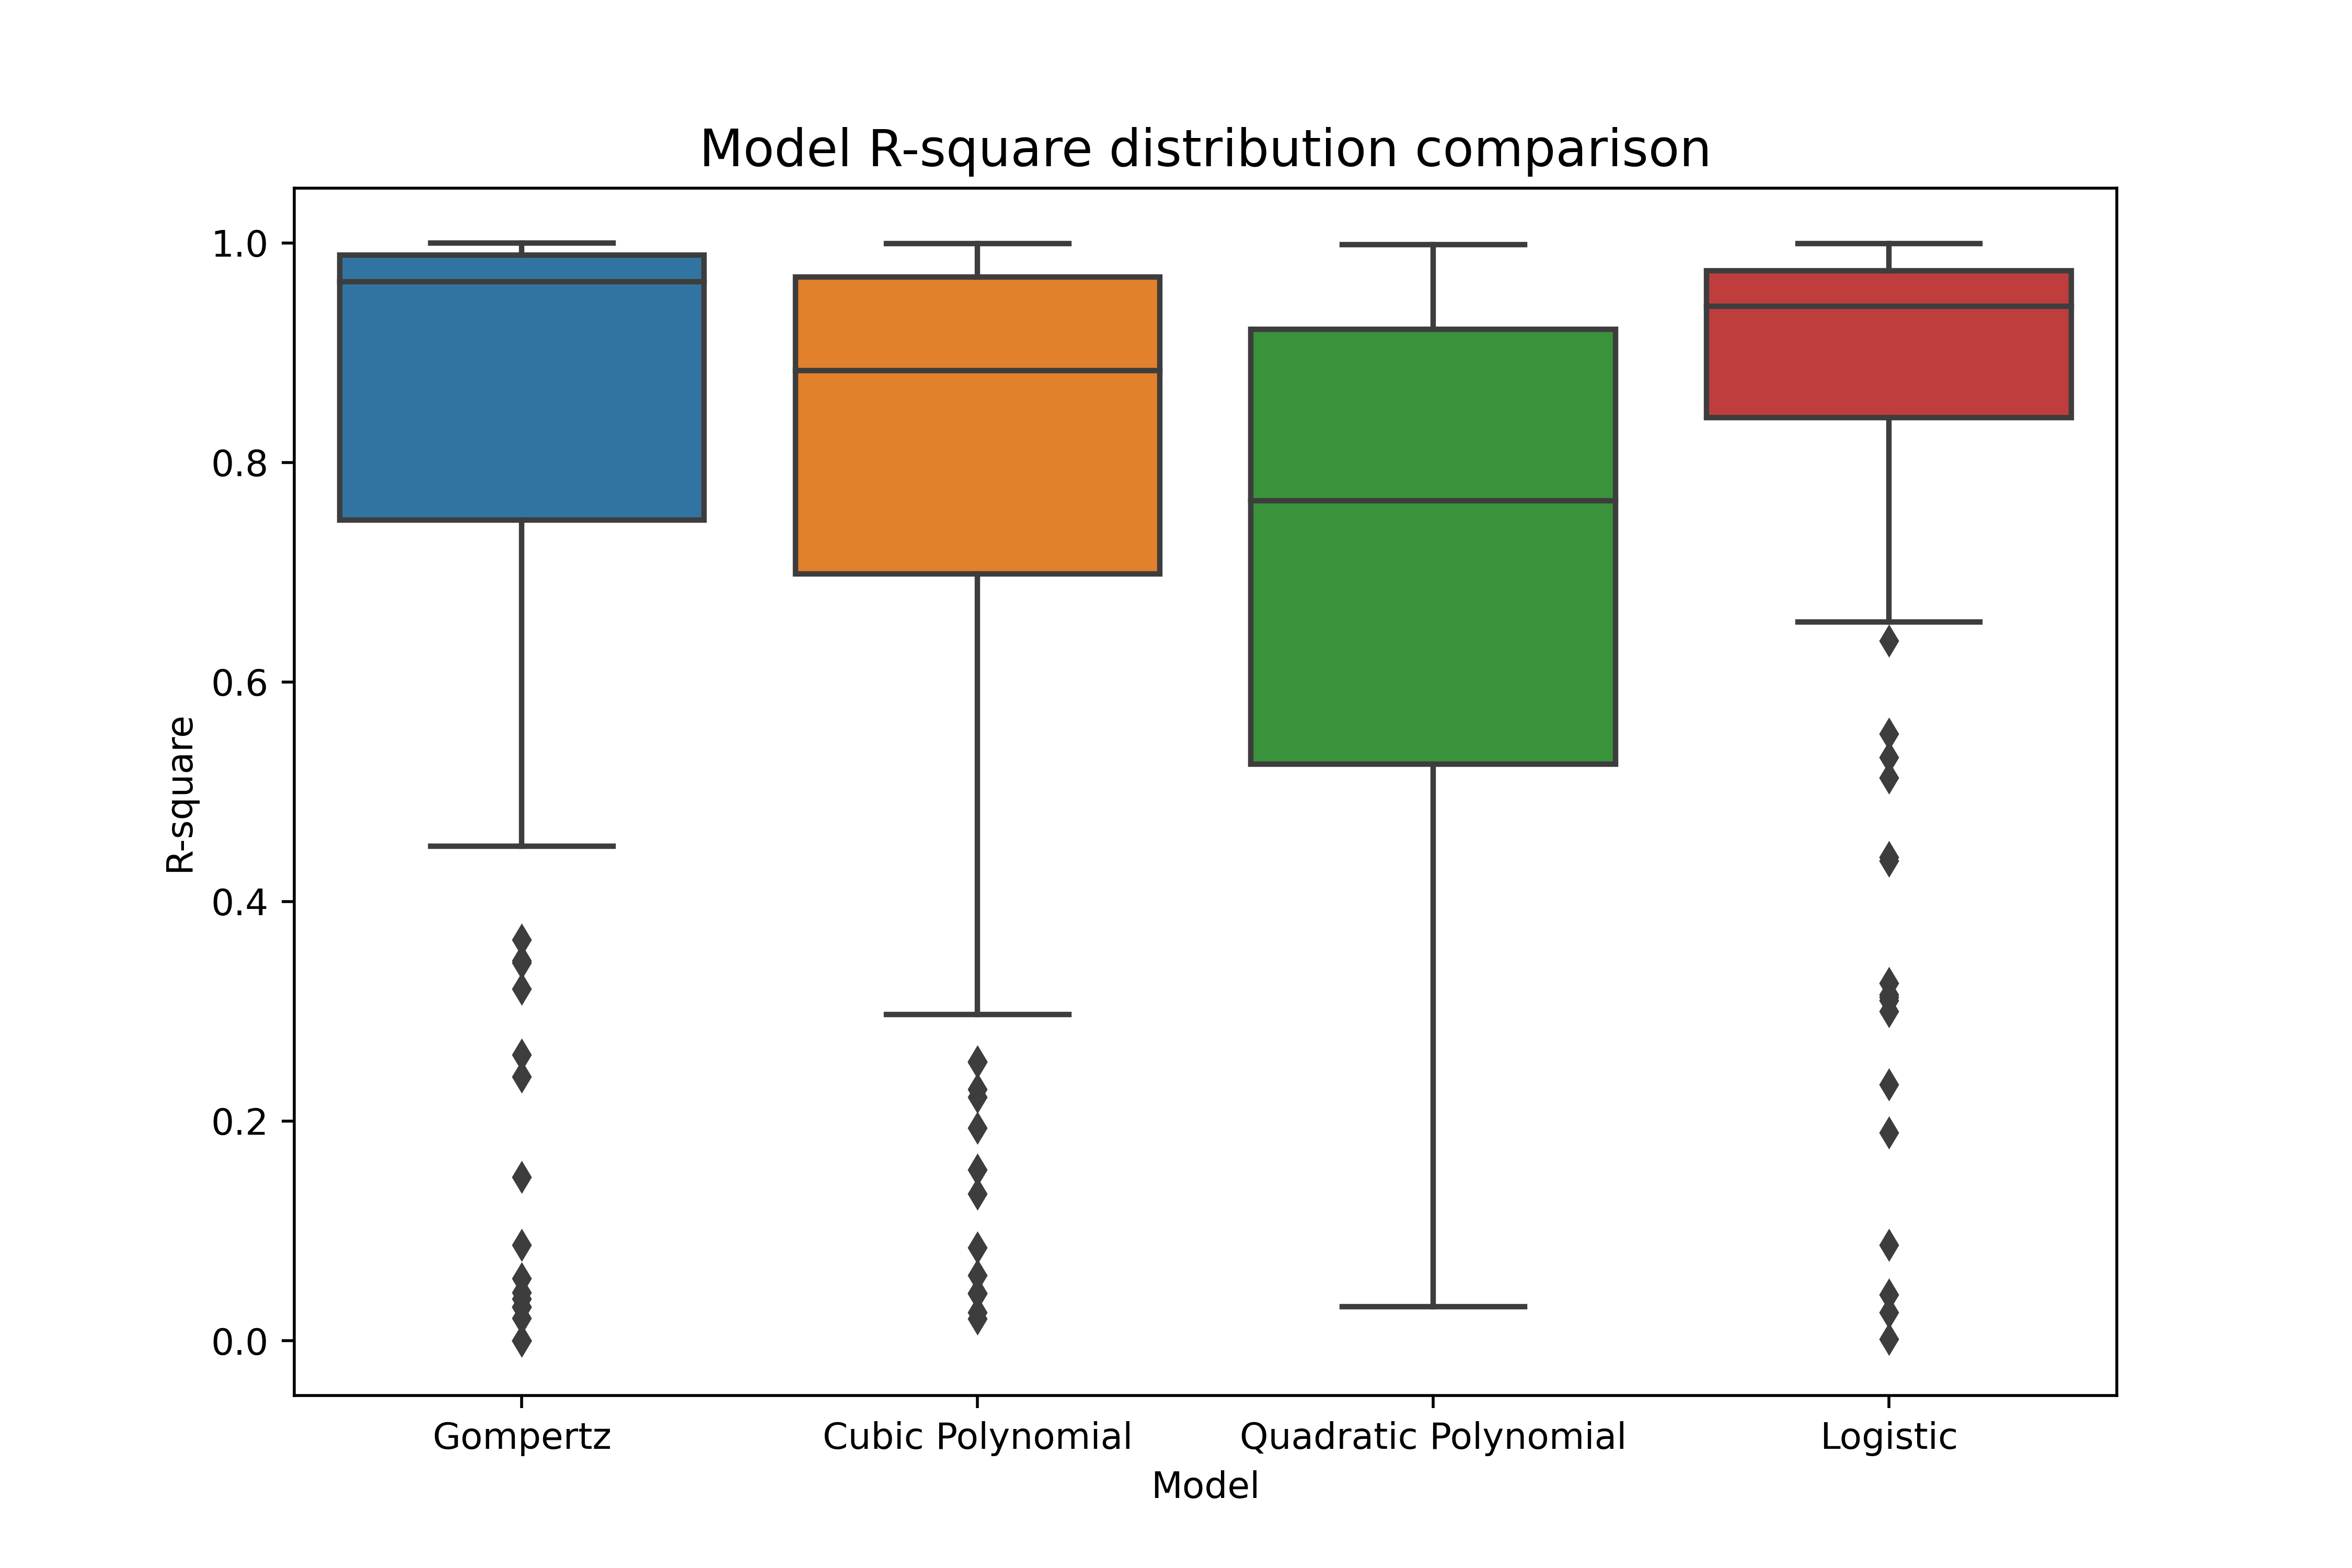
\includegraphics[width=\textwidth]{../results/Model_R2_distribution.png}
      \caption{It showed the $R^2$ distribution}
    \end{figure}

    \begin{figure}[H]
      \centering
      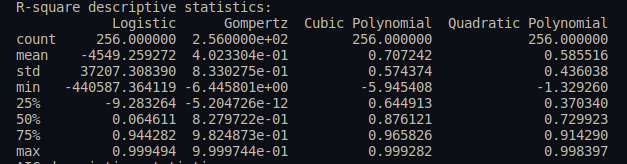
\includegraphics[width=\textwidth]{../sandbox/R-square descriptive statistics.png}
      \caption{It showed the $R^2$ descriptive statistics}
    \end{figure}

    Figure 4 showed the $AIC$ distributions of models. Figure 5 shows the descriptive statistics of $AIC$.
    By comparing the $AICC$ of the models, it illustrated that the Gompertz is the best.

    \begin{figure}[H]
      \centering
      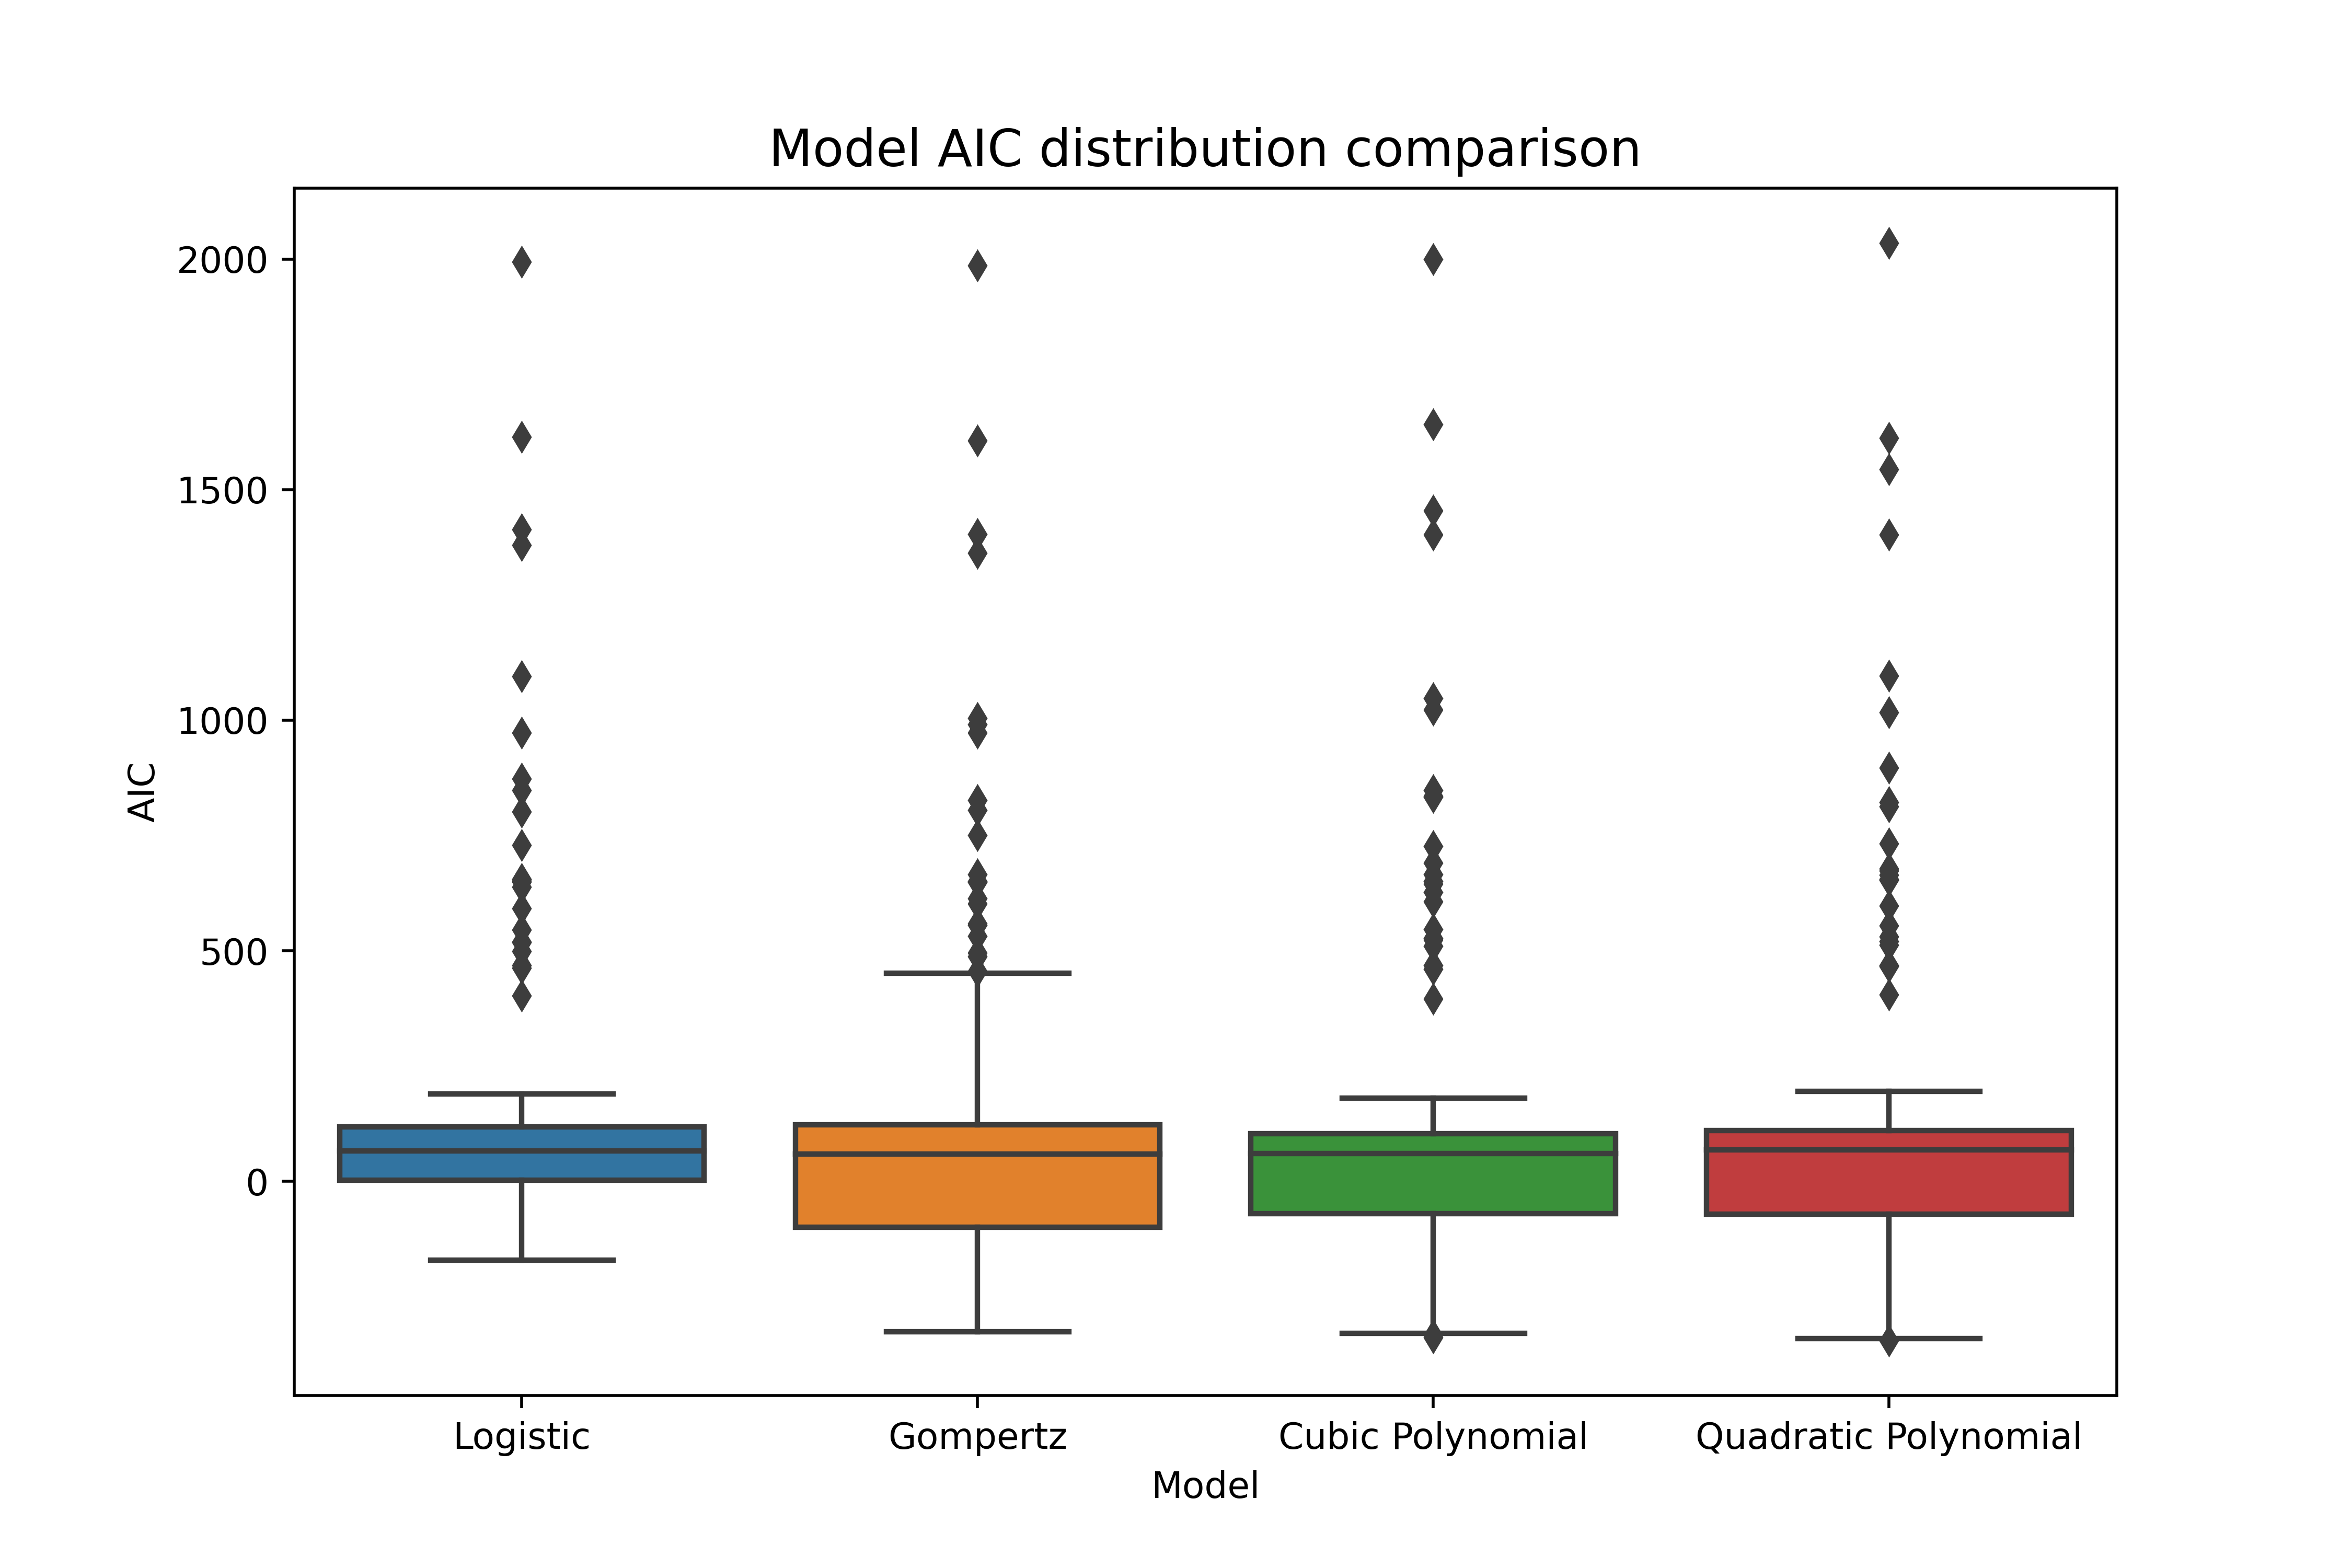
\includegraphics[width=\textwidth]{../results/Model_AIC_distribution.png}
      \caption{It showed the $AIC$ distribution}
    \end{figure}

    \begin{figure}[H]
      \centering
      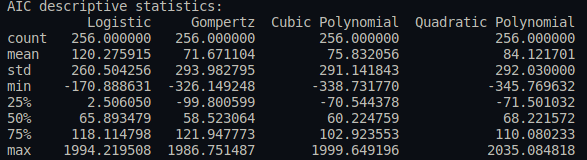
\includegraphics[width=\textwidth]{../sandbox/AIC descriptive statistics.png}
      \caption{It showed the $AIC$ descriptive statistics}
    \end{figure}

    Figure 6 showed the $AIC_c$ distributions of models. Figure 7 shows the descriptive statistics of $AIC_c$. 
    By comparing the $AIC_c$ of the models, it illustrated that the Gompertz is the best.

    \begin{figure}[H]
      \centering
      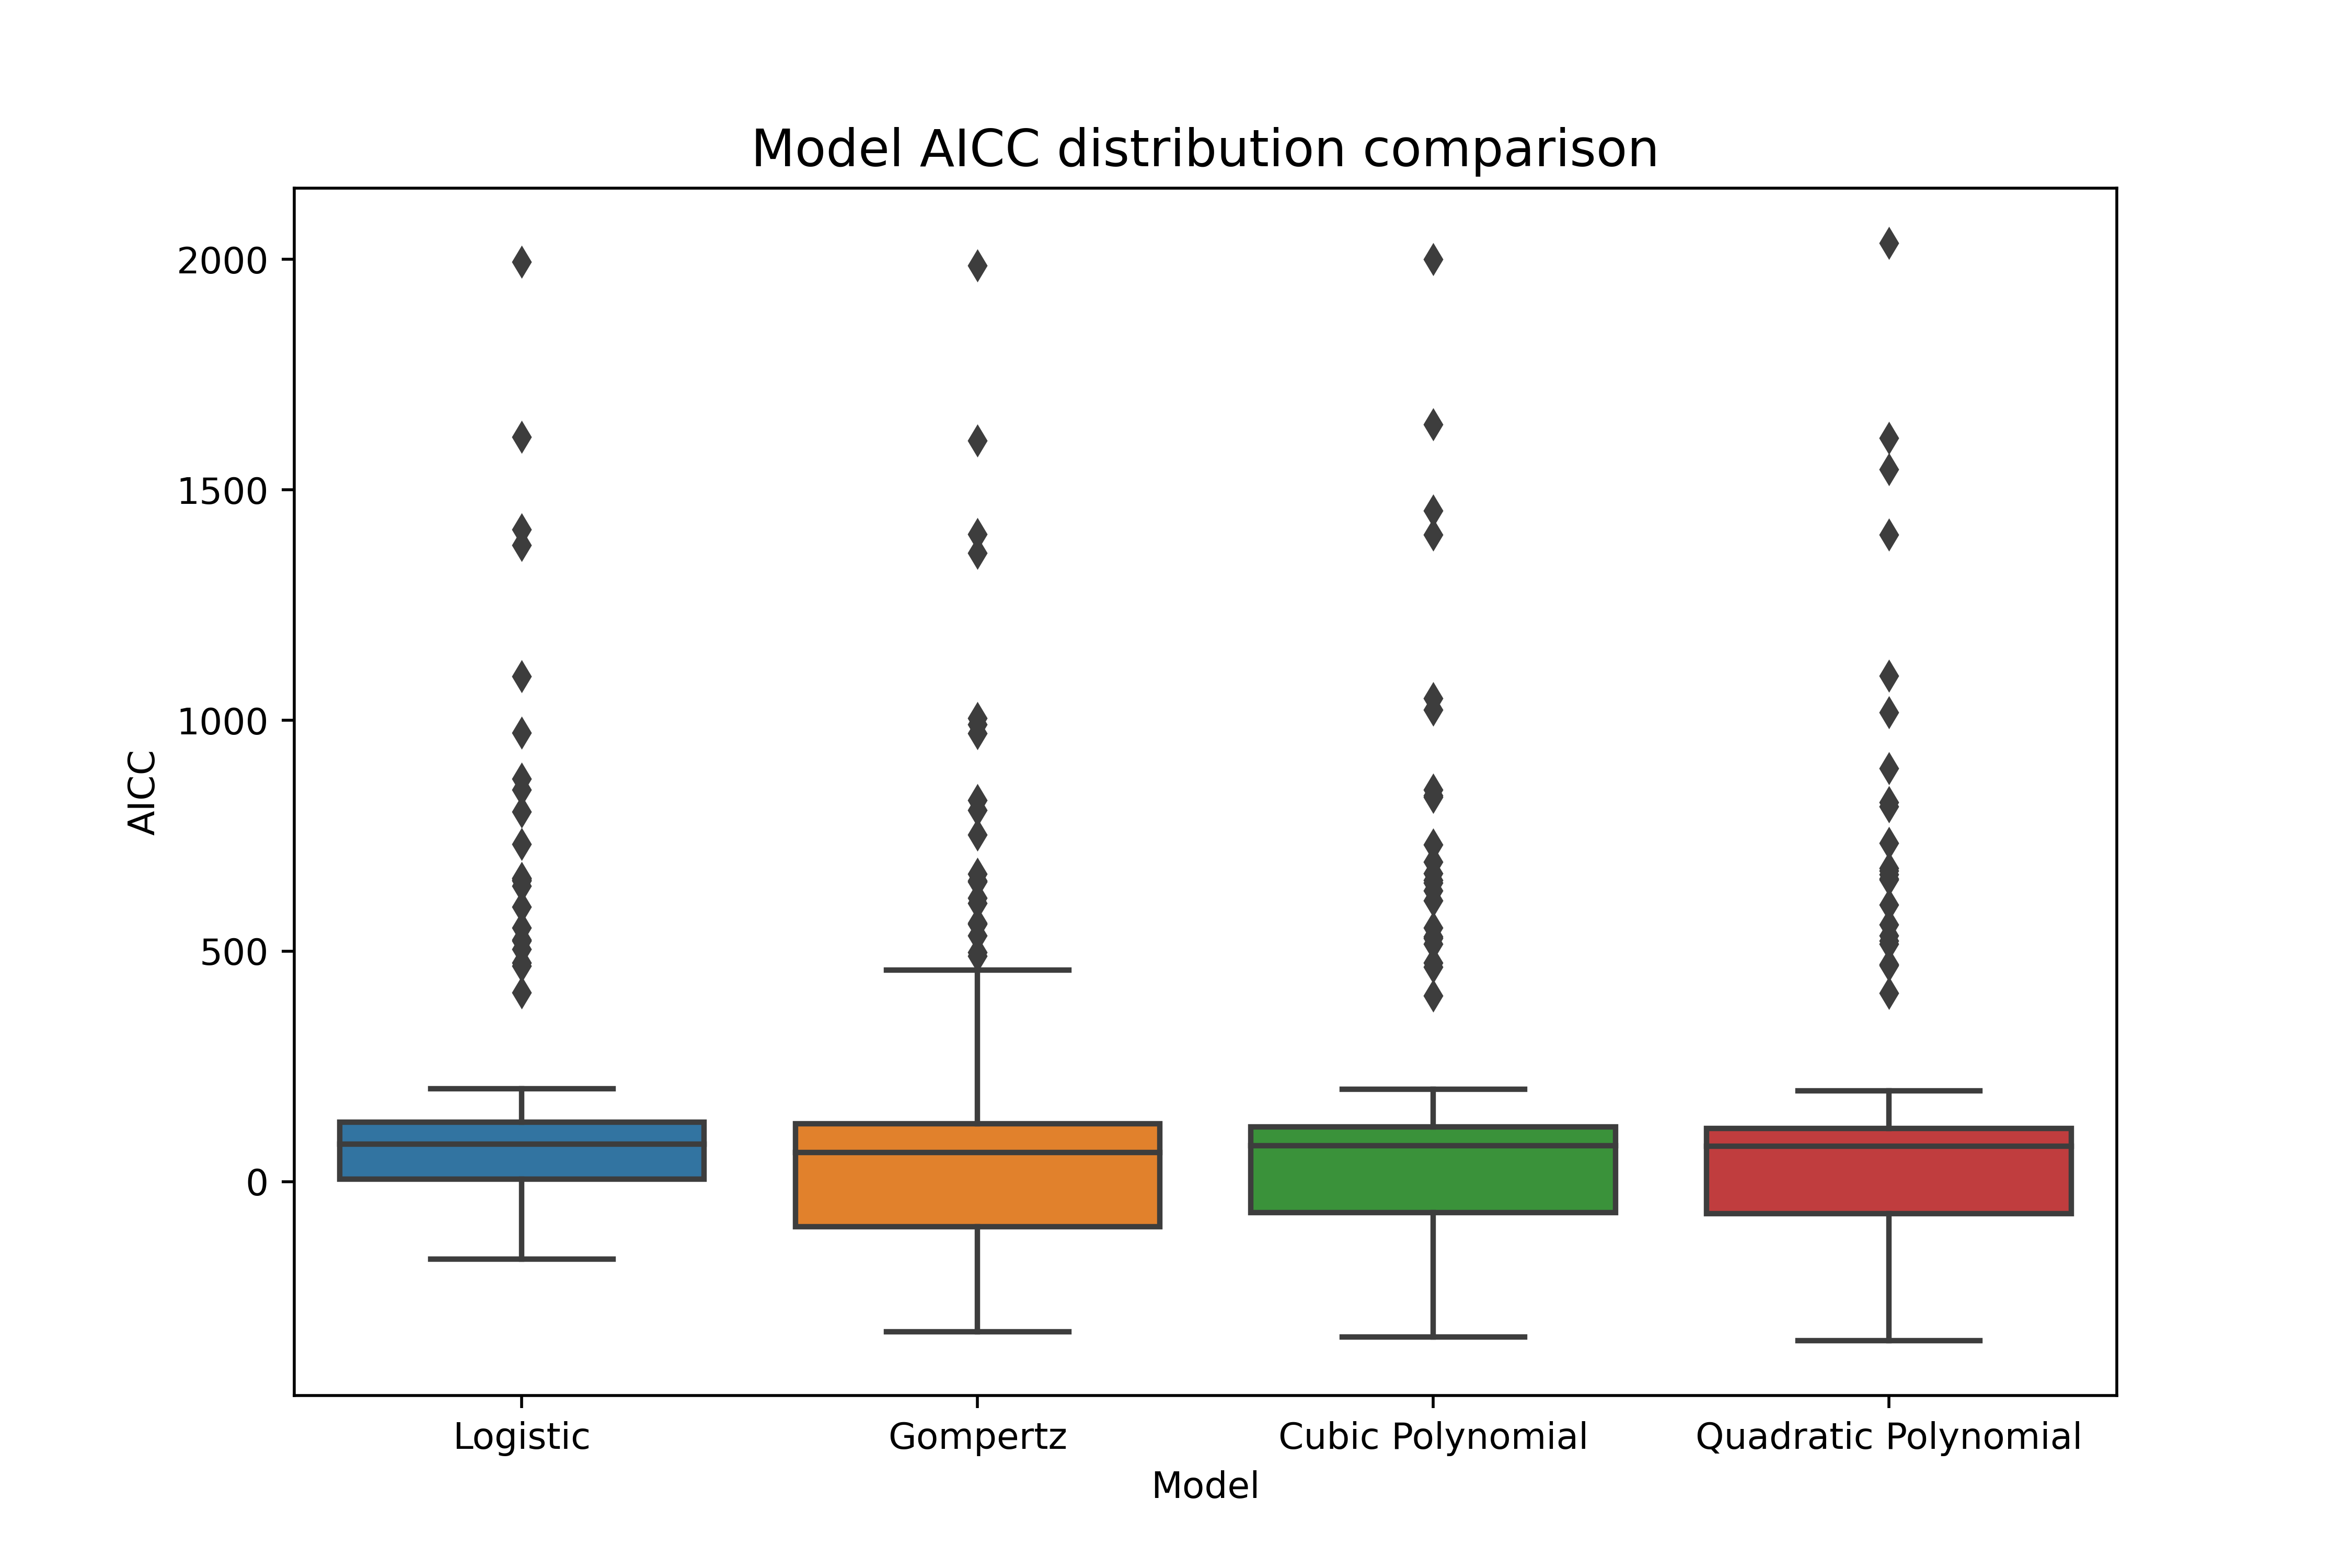
\includegraphics[width=\textwidth]{../results/Model_AICC_distribution.png}
      \caption{It showed the $AIC_c$ distribution}
    \end{figure}

    \begin{figure}[H]
      \centering
      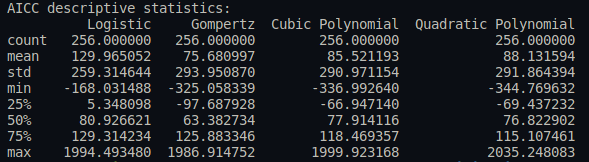
\includegraphics[width=\textwidth]{../sandbox/AICC descriptive statistics.png}
      \caption{It showed the $AIC_c$ descriptive statistics}
    \end{figure}

    Figure 8 showed the $AIC$ distributions of IDs. Figure 9 shows the $AIC_c$ distributions of IDs. 
    These two figures showed the performance of model fitting of different sets.

    \begin{figure}[H]
      \centering
      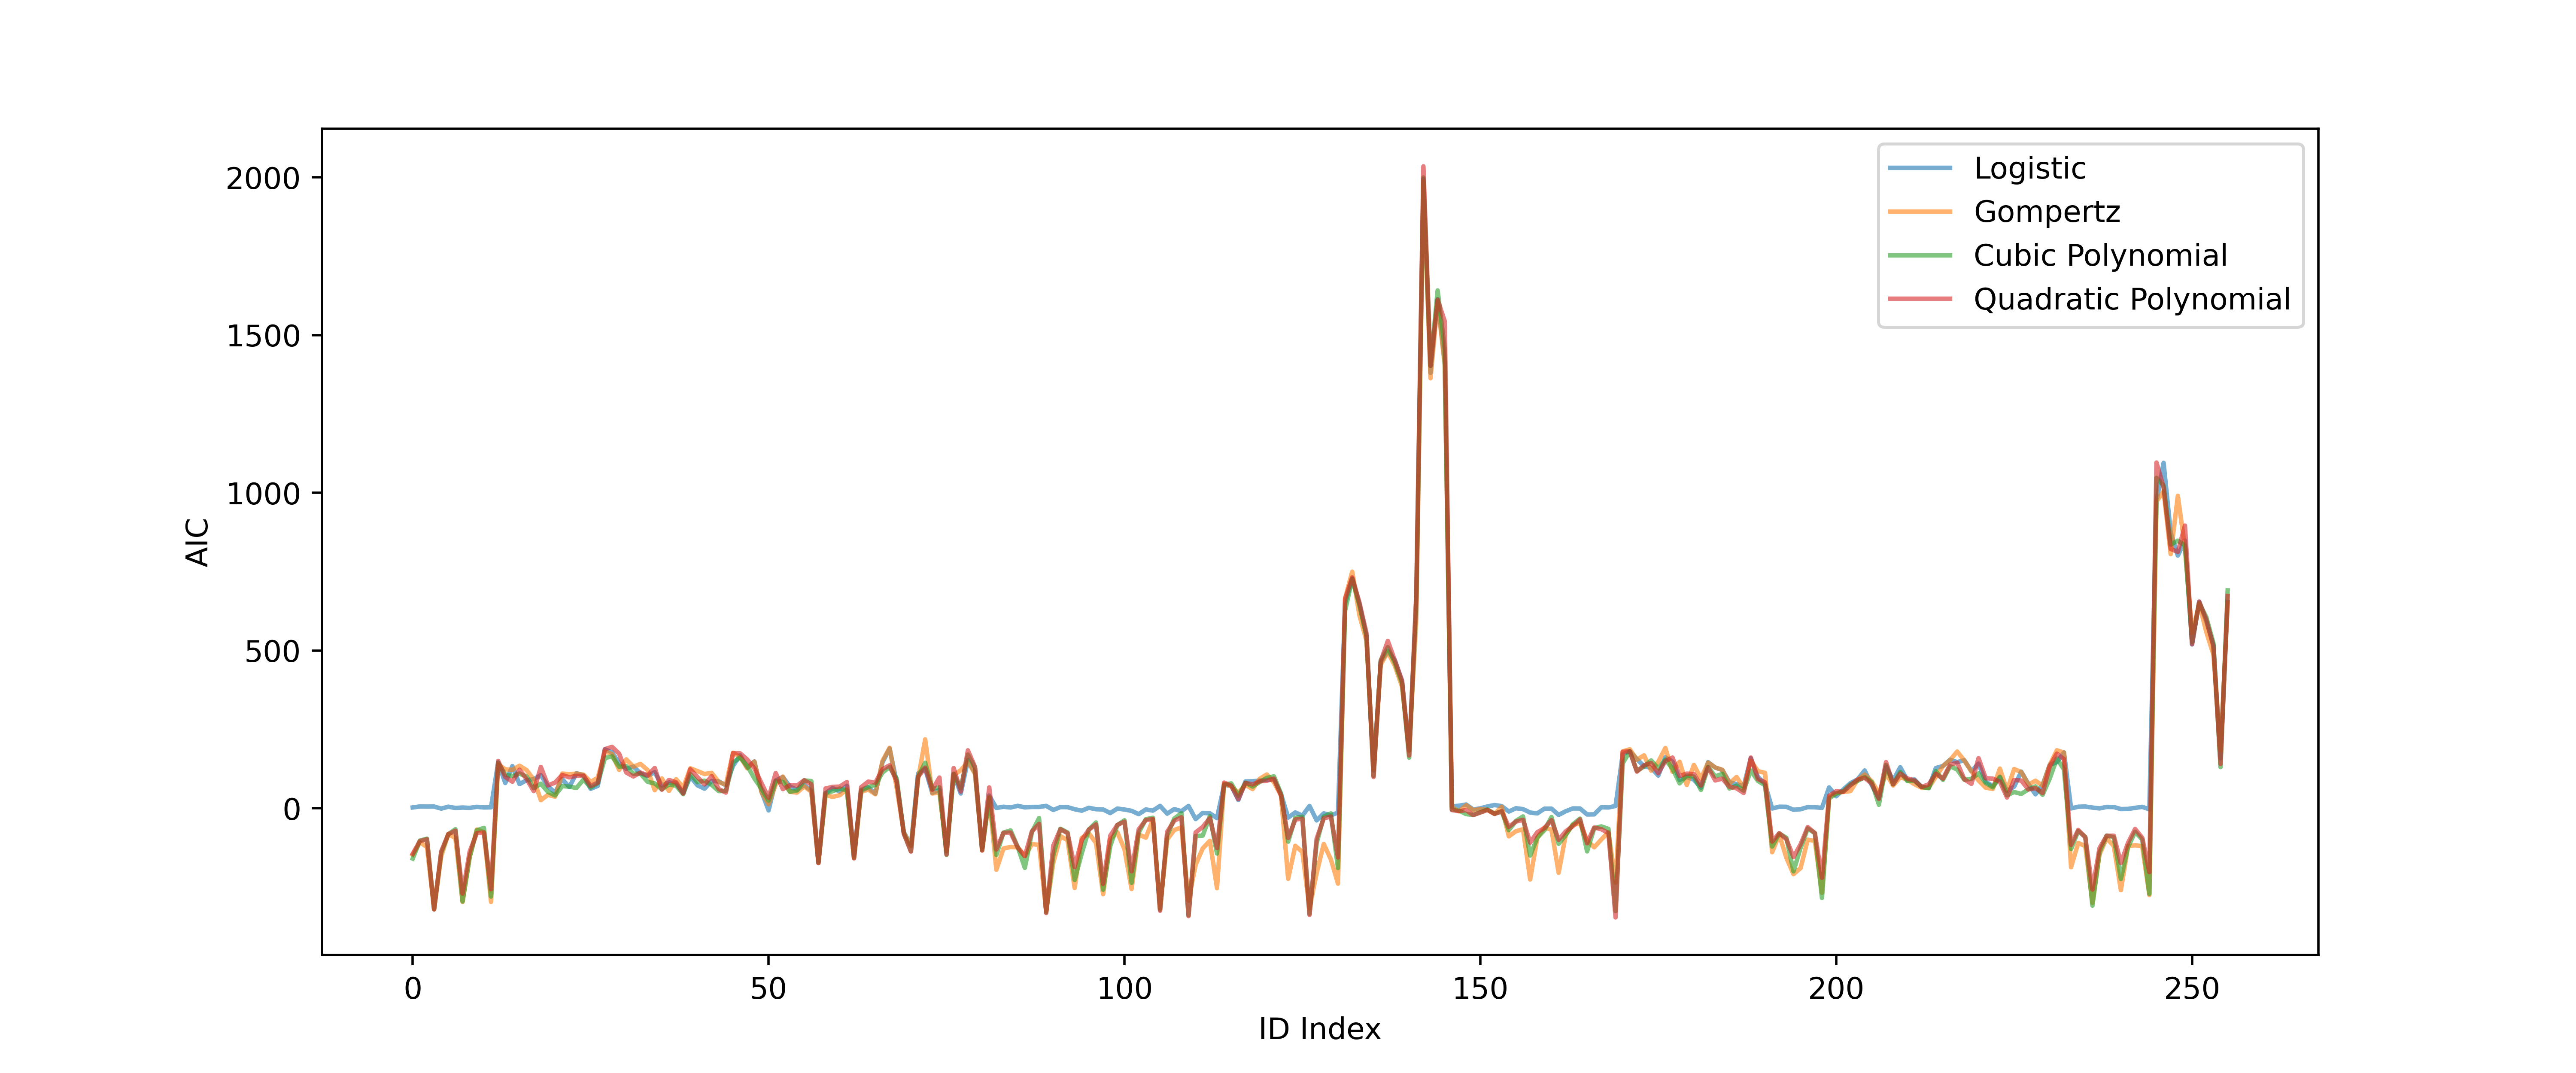
\includegraphics[width=\textwidth]{../results/ID_AIC_distribution.png}
      \caption{It showed the $AIC$ distribution of IDs}
    \end{figure}

    \begin{figure}[H]
      \centering
      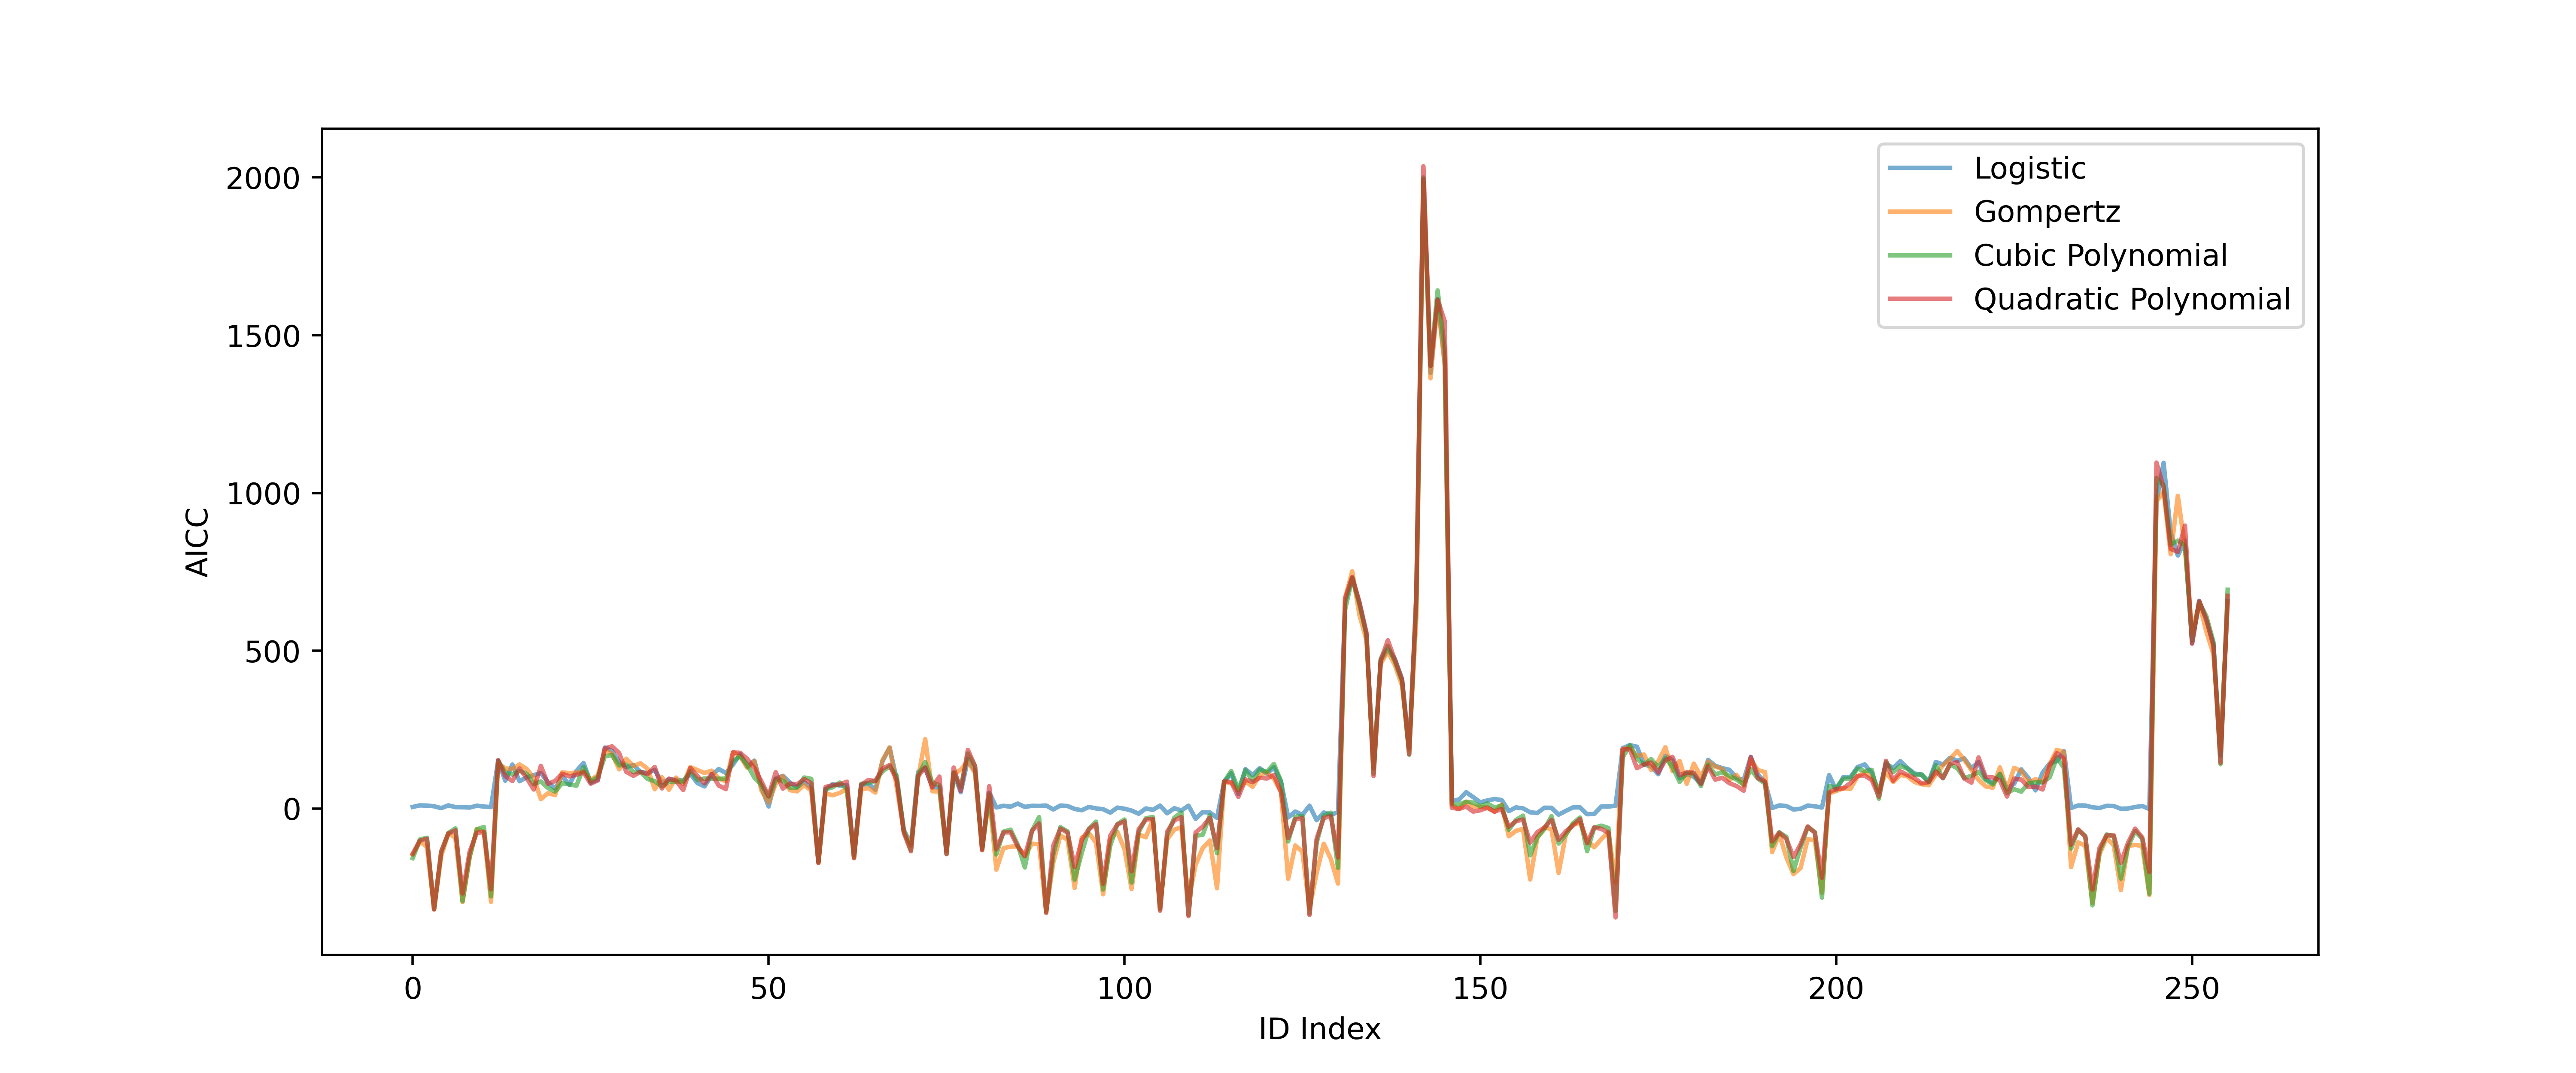
\includegraphics[width=\textwidth]{../results/ID_AICC_distribution.png}
      \caption{It showed the $AIC_c$ distributions of IDs}
    \end{figure}

    

\newpage
\section{Discussion}
The main purpose of this project is to compare OLS with NLLS models and determine which models have the best performance on fitting the specific data (Microbial Population Growth Data).
According to the study, the Cubic Polynomial and Quadratic Polynomial have few parameters with low model complexity, so they fit on most of the data sets. Meanwile, When using $R^2$, a basic statistical evaluation method, OLS stands out. 
Comparing the mean $R^2$ of the four models, $Cubic(0.702)$ is significantly larger than the other models and closest to 1. $Logistic(R^2=-4549.25)$ performed terrible because of the huge amount of unfitted data. 
As those are machine learning models, if each set has more data points, it would greatly improve the accuracy and fitting ability of the models.
However, apart from the non-fitted cases, the NLLS showed promising features. Whether comparing $AIC$ or $AIC_c$, Gompertz model showed the best performance on fitting the data. In $AIC$, $Gompertz(71.67) < Cubic(75.83) < Quadratic(84.12) < Logistic(120.27)$. And in $AIC_c$, $Gompertz(75.68) < Cubic(85.52) < Quadratic(88.13) < Logistic(129.96)$
That is to say, Gompertz should be preferred if extreme performance is sought, as the model has more parameters and a relatively low probability of convergence, it may require more potential labor costs to adjust the initial values.
\newline
In conclusion, NLLS generally outperform OLS for quantifying microbial population growth data. Logistic model is sufficient for the simple growth case. Gompertz model is sufficient for the complex situation as it has the best performance. However,OLS models have advantages as well, they are suitable for simple cases. 
In order to get better performance for Gompertz, it takes more time to optimize it by adjusting the initial values.



\newpage
\bibliographystyle{plain}
\bibliography{References}
\end{document}